
\section{Introduction}
<Write the Introduction>

\section{Technical Part}

\subsection{
    Hardware setups
}

\subsection{
    Breathing rate estimation algorithm
}

\subsection{
    Motion detection algorithm
}

The motion detection via CSI data is based on the statistical electromagnetic model proposed by \cite{LaowuMotionStatistics2019}. For conciseness, we omit the details of the electromagnetic model, but focus on the motion detection based on the motion statistics. 
\par Suppose the CSI data collected is indexed by $H(t, f)$, while we omit other parameters in the dataframe. The corresponding power response $G(t, f) = |H(f, t)|^2$. 
\par We use the sample auto-covariance function $\hat{\gamma}_G(\tau, f)$ where $\tau$ is the lag (c.f. Eqn. (2) in \cite{LaowuMotionStatistics2019}), which is defined as 
$$
\hat{\gamma}_G(\tau, f) = \frac{1}{T} \sum_{t = \tau+1}^{T} (G(t-\tau, f) - \overline{G}(f))(G(t, f) - \overline{G}(f)),
$$
where $T$ is the number of samples (within a window). The ACF of $G(t, f)$ characterized by the lag $\tau > 0$ is defined as
$$
\rho_{G}(\tau, f) = \frac{\hat{\gamma}_G(\tau, f)}{\hat{\gamma}_G(0, f)}.
$$
Whenever the calculation of $\rho_{G}(\tau, f)$ fails, we discard this subcarrier.
The motion detection is performed by hypothesis testing. Denote the set of subcarriers as $\mathcal{F}$, for each $f \in \mathcal{F}$, define the \textbf{motion statistic} as 
$$
\phi(f) = \rho_G\left(\frac{1}{F_s}, f \right).
$$
To perform the following hypothesis testing:
$$
\begin{aligned}
    &H_0: & \hat{\phi}(f) \sim \mathcal{N}(-1/T, 1/T), \quad \forall f \in \mathcal{F}, \\
    &H_1: &\hat{\phi}(f) \xrightarrow{\tau \to 0} \eta(f) > 0, \quad \forall f \in \mathcal{F}.
\end{aligned}
$$
We use the motion statistic estimator
$$
\hat{\psi} = \frac{1}{|\mathcal{F}|} \sum_{f \in \mathcal{F}} \hat{\phi}(f)
$$
to detect the motion, and the decision rule for motion (1) or static (0) is given by $\mathbb{I}\left\{ \hat{\psi} > \eta  \right\}$ for some appropriate choice of parameter $\eta$.





\section{Evaluation}

\subsection{Evaluation Result}
% You should enter your results of the \textbf{evaluation dataset} of both tasks in the table \ref{eval}, e.g., accuracy for motion detection, and median MAE for breathing rate estimation.

<Write your analysis>

\begin{table}[!h]
\centering
\caption{Overall Evaluation Result.}
\label{eval}
    \begin{tabular}{cc}
    \toprule
    \textbf{Evaluation Dataset} & \textbf{Result} \\
    \midrule
    Motion Detection & \textcolor{red}{awaiting test} \\
    Breathing Rate Estimation & <Your median MAE (BPM)> \\
    \bottomrule
    \end{tabular}
\end{table}

\subsection{Benchmark Result}
\subsubsection{Breathing Rate Test}
% You should plot three figures, e.g., Fig.\ref{res1}-\ref{res3}, of your estimated breathing rate, whose titles are the three test files, and put them here.

<Write your analysis>
\begin{figure}[!h]
    \centering
    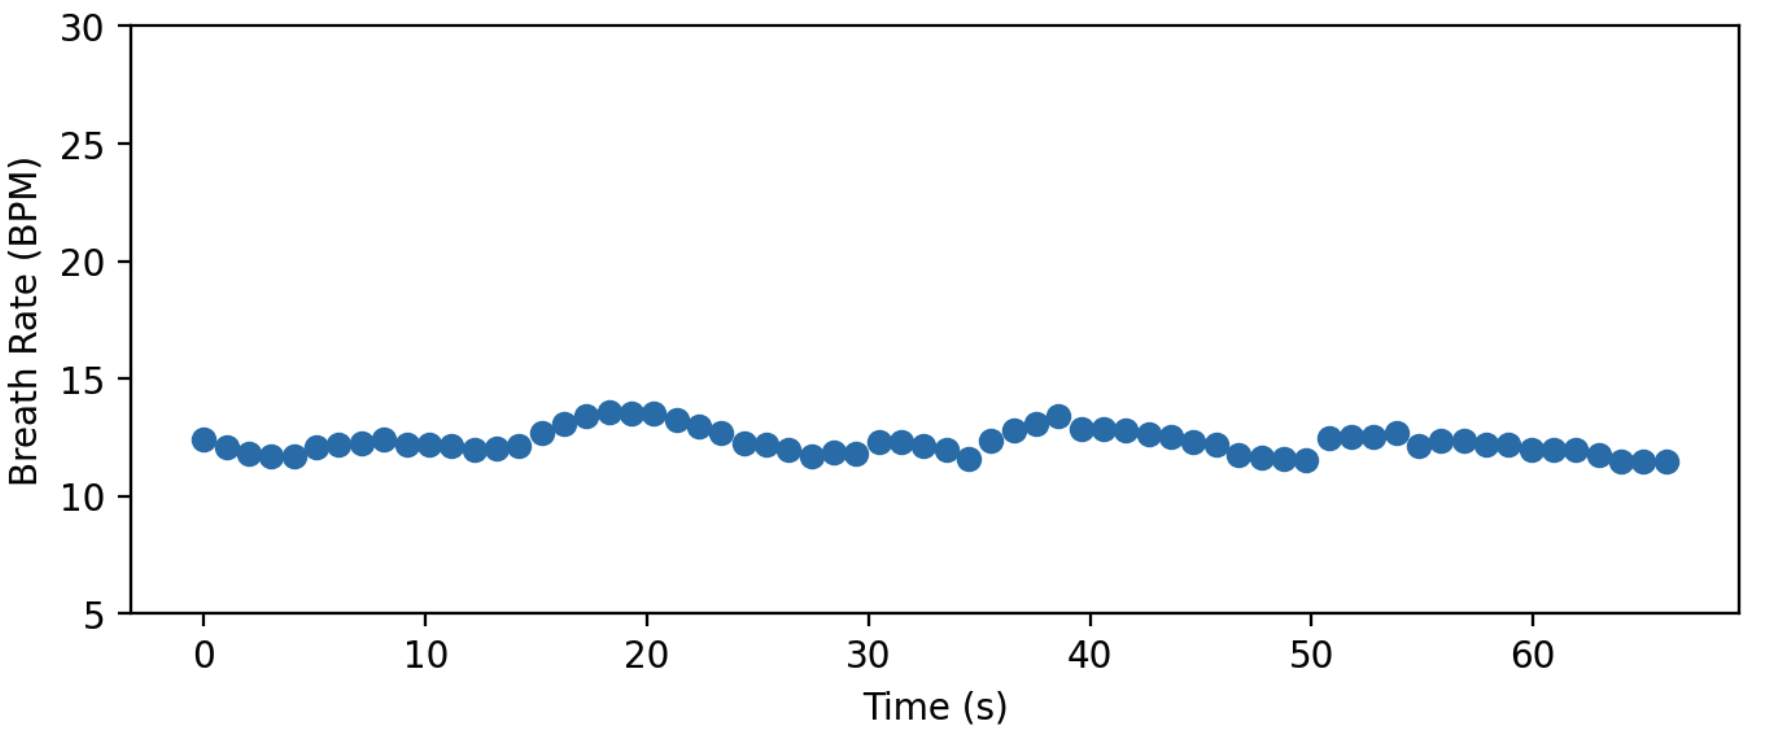
\includegraphics[width=0.5\linewidth]{fig/Exp.jpg}
    \caption{Estimated Respiration for \rm{193342.csv}.}
    \label{res1}
\end{figure}

\begin{figure}[!h]
    \centering
    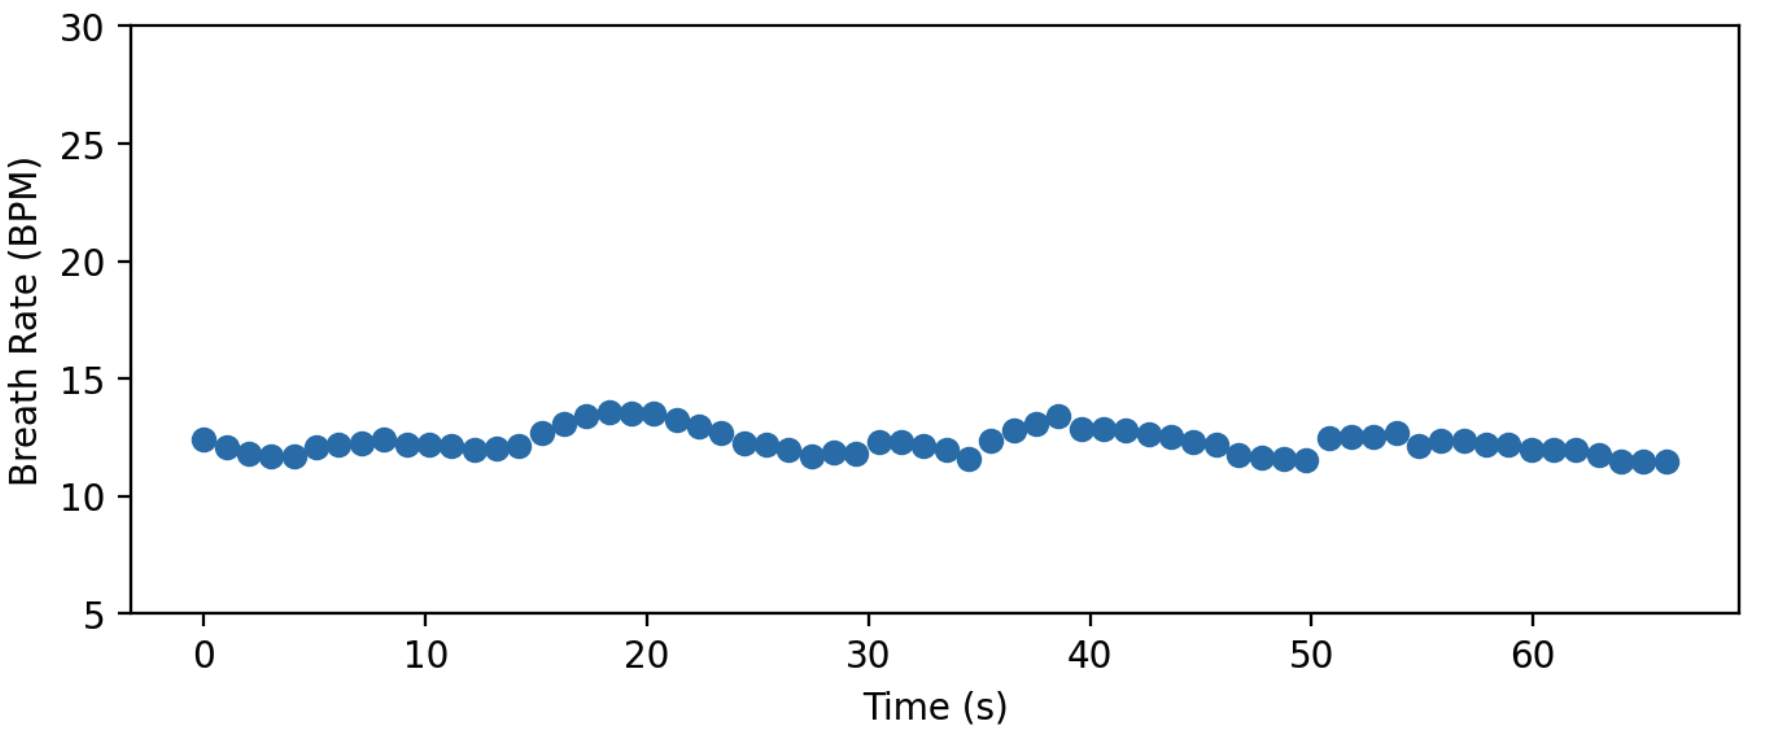
\includegraphics[width=0.5\linewidth]{fig/Exp.jpg}
    \caption{Estimated Respiration for \rm{200223.csv}.}
    \label{res2}
\end{figure}

\begin{figure}[!h]
    \centering
    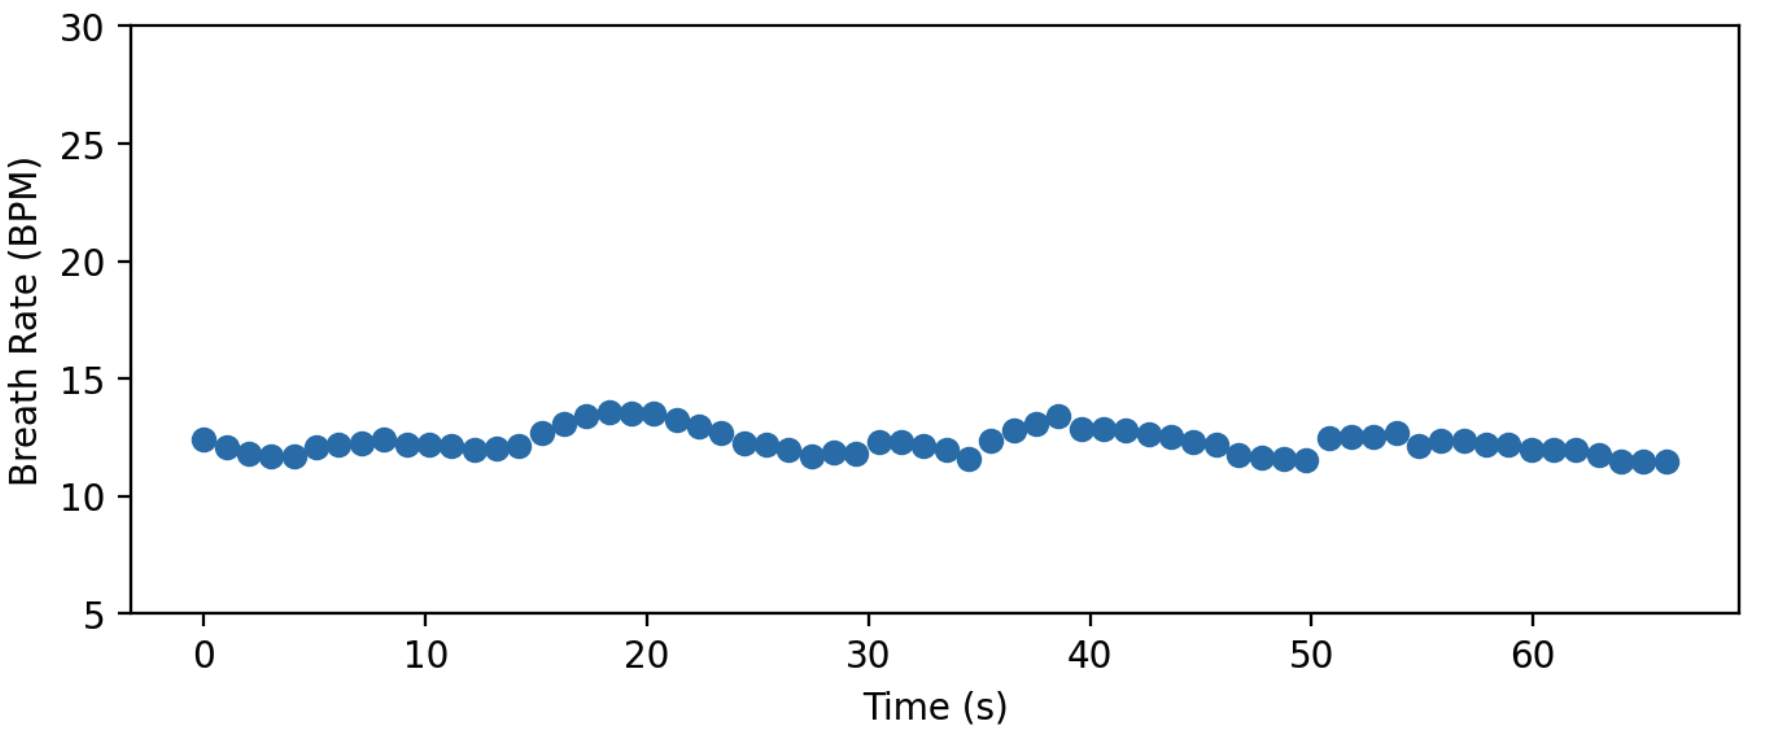
\includegraphics[width=0.5\linewidth]{fig/Exp.jpg}
    \caption{Estimated Respiration for \rm{201424.csv}.}
    \label{res3}
\end{figure}

\subsubsection{Motion Test}
% Enter your result (1 for motion detected, 0 for no) in the table \ref{test motion}.

\begin{table*}[htbp]
    \centering
    \caption{Test result of motion detection with ground truth motion.}
    \label{table:motion_detection_motion}
        \begin{tabular}{cc|cc}
        \toprule
        \textbf{File Name} & \textbf{Result} & \textbf{File Name} & \textbf{Result} \\
        \midrule
        CSI\_20250220\_204932.csv & 100\% & CSI\_20250220\_205516.csv & 100\%\\
        CSI\_20250220\_205301.csv & 100\% & CSI\_20250220\_205526.csv & 100\%\\
        CSI\_20250220\_205318.csv & 100\% & CSI\_20250220\_205539.csv & 100\%\\
        CSI\_20250220\_205330.csv & 100\% & CSI\_20250220\_205553.csv & 100\%\\
        CSI\_20250220\_205343.csv & 100\% & CSI\_20250220\_205607.csv & 100\%\\
        CSI\_20250220\_205356.csv & 100\% & CSI\_20250220\_205624.csv & 100\%\\
        CSI\_20250220\_205406.csv & 100\% & CSI\_20250220\_205637.csv & 100\%\\
        CSI\_20250220\_205439.csv & 80\%  & CSI\_20250220\_205645.csv & 100\%\\
        CSI\_20250220\_205451.csv & 100\% & CSI\_20250220\_205654.csv & 100\%\\
        CSI\_20250220\_205504.csv & 100\% & CSI\_20250220\_205704.csv & 100\%\\
        \bottomrule
        \end{tabular}
    \end{table*}
    
    \begin{table*}[htbp]
        \centering
        \caption{Test result of motion detection with ground truth static.}
        \label{table:motion_detection_static}
            \begin{tabular}{cc|cc}
            \toprule
            \textbf{File Name} & \textbf{Result} & \textbf{File Name} & \textbf{Result} \\
            \midrule
            CSI\_20250220\_203408.csv & 100\% & CSI\_20250220\_210747.csv & 100\%\\
            CSI\_20250220\_204824.csv & 100\% & CSI\_20250220\_210802.csv & 100\%\\
            CSI\_20250220\_210608.csv & 100\% & CSI\_20250220\_210814.csv & 100\%\\
            CSI\_20250220\_210623.csv & 80\% & CSI\_20250220\_210840.csv & 100\%\\
            CSI\_20250220\_210645.csv & 100\% & CSI\_20250220\_210854.csv & 100\%\\
            \bottomrule
            \end{tabular}
        \end{table*}

We conduct the motion detection test on all the csv files contained in directory \texttt{benchmark/motion\_de} \texttt{tection/evaluation\_motion} and \texttt{evaluation\_static}. As each csv contains 300 samples, the sampling rate $F_s$ is 100Hz, we set the windows size to be 100, step size to be 50, the lag $\tau = 1$, and the threshold $\eta = 0.4$. The algorithm reports an accuracy of 98\% on static benchmark and 99\% on motion benchmark. Accuracy on each testcase is reported in \autoref{table:motion_detection_motion} and \autoref{table:motion_detection_static}.





\section{Conclusion}



%%%%%%%%%%%%%%%%%%%%%%%%%%%%%%%%%%%%%%%%%%%%%%
% The following sections are excluded from the page limit
%%%%%%%%%%%%%%%%%%%%%%%%%%%%%%%%%%%%%%%%%%%%%%
\appendix
\section{Appendix I}
\subsection{Individual Contribution}
% You should list the contribution and statements in the table \ref{individual contribution}.

\begin{table*}[!h]
\centering
\caption{Individual Contribution}
\label{individual contribution}
    \begin{tabular}{ccc}
    \toprule
    \textbf{Name} & \textbf{UID} & \textbf{Contribution Statement} \\
    \midrule
    A & a & a\%, a's role and contributions here. \\
    B & b & b\%, b's role and contributions here. \\
    C & c & c\%, c's role and contributions here. \\
    D & d & d\%, d's role and contributions here. \\
    \bottomrule
    \end{tabular}
\end{table*}

%%%%%%%%%%%%%%%%%%%%%%%%%%%%%%%%%%%%%%%%%%%%%5
% replace \hspace{1em} with 1 or 0
\subsection{Checklist of your submission}

\begin{table*}[!h]
\caption{Self-Report Submission Checklist (1=Done, 0=No)}
\label{tab:checklist}
\begin{tabularx}{\textwidth}{L C}
\toprule
\textbf{Items} & \textbf{Status} \\
\midrule

Successfully receive the CSI data. & \underline{\hspace{1em}} \\
Successfully transmit the data over MQTT. & \underline{\hspace{1em}} \\
The algorithm is implemented on-board. & \underline{\hspace{1em}} \\
The algorithm is implemented in real-time. & \underline{\hspace{1em}} \\
Successfully develop an end-to-end system for data visualization. & \underline{\hspace{1em}} \\
\midrule

Submit the video (no more than 3 minutes). & \underline{\hspace{1em}} \\
The submitted files contain all code necessary to reproduce and verify the results, ensuring full reproducibility of the work. & \underline{\hspace{1em}} \\
\midrule

We confirm that all data results are consistent with the code execution outcomes. & \underline{\hspace{1em}} \\
We confirm that the contribution statement is accurate and that there are no objections from any team members. & \underline{\hspace{1em}} \\
We acknowledge the use of GenAI and ensure that it has been correctly cited or referenced in accordance with the required guidelines. & \underline{\hspace{1em}} \\
We certify that all information in this checklist is accurate, complete, and compliant with academic integrity policies. & \underline{\hspace{1em}} \\

\bottomrule
\end{tabularx}
\end{table*}
% add whatever you want
\section{Appendix II}


